\documentclass[a4paper,11pt]{book} % Tamaño de papel, tamaño de letra y clase LaTeX usada...

\usepackage[spanish]{babel} % Permite escribir en Castellano (tildes y ñ) e implementa...
\usepackage[utf8]{inputenc} % Permite introducir acentos y Ñ directamente.
%\usepackage[T1]{fontenc} %permite cambiar la fuente por defecto.
\usepackage{bm} % Permite letras griegas en negrita {uso: \bm{\alpha}}
\usepackage{graphicx}
\usepackage{amssymb}
\usepackage{mathtools}
\usepackage{subfigure}
\usepackage{multicol} %para añadir texto en columnas
\usepackage{float}
\usepackage{fancyhdr} %encabezados y pies de pagina
\usepackage{amsmath,amsfonts,latexsym,color,textcomp,anysize}
\usepackage[table,xcdraw]{xcolor}
\usepackage{longtable}
\usepackage{parskip}
\usepackage{hyperref}
\usepackage{cancel} % tachar cosas \cancel{}
%\usepackage{tensor} % Notación: \tensor{T}{^a_b^c_d}
%\usepackage{mathrsfs}
\usepackage{slashed}   %\slashed{p}
\spanishdecimal{.}
\usepackage{cite}
%\usepackage[style=numeric-comp]{biblatex}
\usepackage{yhmath}
\usepackage[left=2.00cm, right=2.00cm, top=0cm, bottom=2cm,
includehead, nomarginpar, headheight=2.5cm, headsep=0.3cm
%includefoot,
%textwidth=10cm,% Set \textwidth to 10cm
]{geometry}

\hypersetup{
    colorlinks=true,
    linkcolor=blue,
    filecolor=magenta,      
    urlcolor=cyan}

\usepackage[braket, qm]{qcircuit}

\setcounter{MaxMatrixCols}{12}
\usepackage{changepage}
\usepackage{framed}
\usepackage{caption}
%\usepackage{subcaption}

% =========================================================================================
% Cuadros
\usepackage[most]{tcolorbox}
\tcbuselibrary{listingsutf8}
\newtcolorbox{mybox_blue}[1]
{enhanced jigsaw, breakable, pad at break*=1mm,  colback=cyan!5!white,colframe=cyan!75!black,fonttitle=\bfseries,title=#1}

\newtcolorbox{mybox_green}[1]
{enhanced jigsaw, breakable, pad at break*=1mm, colback=green!5!white,colframe=green!45!black,fonttitle=\bfseries,title=#1}

\newtcolorbox{mybox_red}[1]
{enhanced jigsaw, breakable, pad at break*=1mm, colback=red!5!white,colframe=red!45!black,fonttitle=\bfseries,title=#1}

\newtcolorbox{mybox_orange}[1]
{enhanced jigsaw, breakable, pad at break*=1mm, colback=orange!10!white,colframe=orange!80!black,fonttitle=\bfseries,title=#1}

\newtcolorbox{mybox_gray}[1]
{enhanced jigsaw, breakable, pad at break*=1mm, colframe=gray!45!black}

\newtcolorbox{mybox_gray2}[1] % Sin bordes
{enhanced, sharp corners, breakable, pad at break*=1mm, boxrule=0pt, toprule=1pt, bottomrule=1pt, colframe=black}


% =========================================================================================
% Teoremas, lemas y demostraciones
\newtheorem{lemma_contador}{Lemma}
	\newcommand{\Lemma}[1]{
		\begin{mybox_gray2}{}
			\begin{lemma_contador}
				 #1 
			\end{lemma_contador} 
		\end{mybox_gray2}
	}
	
\newtheorem{teorema_contador}{Teorema}
	\newcommand{\Teorema}[1]{
		\begin{mybox_gray2}{}
			\begin{teorema_contador}
				 #1 
			\end{teorema_contador} 
		\end{mybox_gray2}
	}

\newtheorem{corolario_contador}{Coloralio}
	\newcommand{\Corolario}[1]{
		\begin{mybox_gray2}{}
			\begin{corolario_contador}
				 #1 
			\end{corolario_contador} 
		\end{mybox_gray2}
	}

\newtheorem{definicion_contador}{Definición}
	\newcommand{\Definicion}[1]{
		\begin{mybox_gray2}{}
			\begin{definicion_contador}
				 #1 
			\end{definicion_contador} 
		\end{mybox_gray2}
	}

\newtheorem{proposicion_contador}{Proposición}
	\newcommand{\Proposicion}[1]{
		\begin{mybox_gray2}{}
			\begin{proposicion_contador}
				 #1 
			\end{proposicion_contador} 
		\end{mybox_gray2}
	}

\newtheorem{ejercicio_contador}{Ejercicio}
	\newcommand{\Ejercicio}[1]{
		\begin{mybox_gray}{Ejercicio} 
			\begin{ejercicio_contador}
				 #1 
			\end{ejercicio_contador} 
		\end{mybox_gray}
	}
	
\def\proof{\begin{mybox_gray2} \textbf{\textbf{Demostración: }} } %\def\proof{\paragraph{Demostración: }}
\def\endproof{\hfill$\blacksquare$ \end{mybox_gray2}}

% =========================================================================================
% codigo Python
\usepackage{listings} 	% \begin{lstlisting}
\definecolor{dkgreen}{rgb}{0,0.6,0}
\definecolor{gray}{rgb}{0.5,0.5,0.5}
\definecolor{mauve}{rgb}{0.58,0,0.82}
\lstset{frame=tb,
  language=Python,
  aboveskip=3mm,
  belowskip=3mm,
  showstringspaces=false,
  columns=flexible,
  basicstyle={\small\ttfamily},
  numbers=none,
  numberstyle=\tiny\color{gray},
  keywordstyle=\color{blue},
  commentstyle=\color{dkgreen},
  stringstyle=\color{mauve},
  breaklines=true,
  breakatwhitespace=true,
  tabsize=3
}

%Includes "References" in the table of contents
\usepackage[nottoc]{tocbibind}
%===========================================================================================
%numerar ecuaciones con la seción
\numberwithin{equation}{chapter}

%===========================================================================================
% Margenes, sangria, espacio entre parágrafos

%\marginsize{2cm}{2cm}{2cm}{1.5cm} %MÁRGENES: Izq, Der, Sup, Inf.
\parindent=0mm % Sangría por defecto
\parskip=3mm % Espacio entre párrafos por defecto

%===========================================================================================
% Definiciones de utilidad

% Parentesis
\def\lp{\left(}
\def\rp{\right)}

\def\lc{\left[}
\def\rc{\right]}

\def\lch{\left\{}
\def\rch{\right\}}

\def\l|{\left|}
\def\r|{\right|}

\def\Lp{\Bigl(}
\def\Rp{\Bigr)}

\def\Lc{\Bigl[}
\def\Rc{\Bigr]}

\def\Lch{\Bigl\{}
\def\Rch{\Bigr\}}

\def\L.{\Bigl.}
\def\R.{\Bigr.}

% Cosas cuanticas
\newcommand{\branew}[1]{\langle #1|} 
\newcommand{\ketnew}[1]{|#1\rangle} 
\newcommand{\braket}[2]{\langle #1|#2\rangle} 
\newcommand{\ketbra}[2]{| #1\rangle \! \langle #2|} 
%\newcommand{\ketbra}[2]{| #1\rangle \langle #2|} 
\newcommand{\cg}[1]{{\rm C}#1} 

% Cosas útiles
\def\Nabla{\bm{\nabla}}
\def\rqa{\quad \Rightarrow \quad}
\def\senc{\, \text{senc}}
%===========================================================================================
% Para poner subsubsections en letra pequeña y crear subsubsubsection en letra pequeña

% Subsub en cursiva y subrayado
\def\subsubiContadorIt{\par\addtocounter{subsubsection}{1}\underline{\it\thesubsubsection.}\hskip0.5cm \setcounter{subsubsubsectionIt}{0}}
	\newcommand{\SubsubiIt}[1]{
		\subsubiContadorIt \textit{#1}
	}

% subsubsub con cursita y subrayado
\newcounter{subsubsubsectionIt}[subsubsection]
\def\subsubiiContadorIt{\par\addtocounter{subsubsubsectionIt}{1}\underline{\it \thesubsubsection.\thesubsubsubsectionIt.}\hskip0.5cm}
	\newcommand{\SubsubiiIt}[1]{
		\subsubiiContadorIt \textit{#1}
	}

% subsubsub negrita
\newcounter{subsubsubsectionBf}[subsubsection]\def\subsubiiContadorBf{\par\addtocounter{subsubsubsection_bf}{1}\bf \thesubsubsection.\thesubsubsubsection.\hskip0.5cm}
	\newcommand{\SubsubiiBf}[1]{
		\subsubsubsectionBf \textbf{#1}
	}
%===========================================================================================

%\title{\Huge{\textbf{Introducción a la Computación Cuántica.}}}
%\author{David Castaño Bandín (UMA)}
%\date{Año 2023}
%\newpage

%===========================================================================================
% Logos en todas las páginas

\usepackage{fancyhdr}
\pagestyle{fancy}
\fancyhead{} % clear all header fields
\fancyhead[L]{\nouppercase{\leftmark}}
\fancyhead[R]{
\includegraphics[width=0.2\linewidth]{Figuras/Fig_logo_UMA_positivo.png}}
%\fancyhead[R]{
\includegraphics[width=0.13\linewidth]{Figuras/Fig_logo_scbi.png}}
\fancyfoot{} % clear all footer fields
\fancyfoot[C]{\thepage}
\renewcommand{\headrulewidth}{0.5pt}
\renewcommand{\footrulewidth}{0pt}

% ================================= PORTADA =======================================
%\pagestyle{empty}

\begin{document}
\Ejercicio{
Calcula a mano la forma polar de los números:
\begin{equation}
4 + 3i, \quad 7 - 2i, \quad - 5 + 5i, \quad - 3 + 4i
\end{equation}
}

\Ejercicio{
Demuestra la expresión $A_{ij} = \bra{i} A \ket{j}$. Para ello usa la Ec. (\ref{ec_formalismo_base_operadores})
}

\Ejercicio{
Demuestra este resultado, es decir, demuestra que:
\begin{align*}
(UV)^\dagger & = (UV)^{-1} \\
(U+V)^\dagger & \neq (U+V)^{-1}
\end{align*}
}

\Ejercicio{
Resta de ${\rm dim}_{\bf R}({\rm L}(\mathcal{H})) =  2N^2$ el número de ecuaciones que restringen la matriz de un operador unitario y halla así la dimensión (real) de la \textit{variedad de operadores unitarios}.
}

\Ejercicio{
Resta de $2N^2$ el número de ecuaciones que restringen la matriz de un operador hermítico y halla así la dimensión del \textit{subespacio vectorial hermítico}
}

\Ejercicio{
Demuestra este resultado
}

\Ejercicio{
Comprueba la Ec. (\ref{ec_formalismo_des_espectral}).
}

\Ejercicio{
Escribe la descomposición espectral de las tres matrices de Pauli, $\sigma_x, \sigma_y $ y $\sigma_z$.
}

\Ejercicio{
Demuestra las siguientes relaciones de (anti)conmutación
\begin{equation}
\{\sigma_i,\sigma_j \} = 2\delta_{ij}~~~~~~~,~~~~~~~
~~~[\sigma_i,\sigma_j] = 2i\epsilon_{ijk}\sigma_k
\end{equation}
}

\Ejercicio{
Demuestra estos resultados.
}

\Ejercicio{
Calcula $\sigma_1\otimes \sigma_2\otimes \sigma_3$
}

\Ejercicio{
Considera la base $\{\ket{0},\ket{1} \}$ del espacio $\mathcal{H}$ de dimensión 2. Sea $A= B + C$ un operador que actúa sobre el producto $\mathcal{H}\otimes \mathcal{H}$,  donde $B$ y $C$ son operadores factorizables dados por
\begin{equation}
B = \ketbra{0}{0}\otimes I ~~~, ~~~~
C = \ketbra{1}{1}\otimes (\ketbra{0}{1} + \ketbra{1}{0})
\end{equation}
Escribe los elementos $B_{ij}$ y $C_{ij}, i,j=1,2,3,4$  y obtén $A_{ij}$. Comprueba si $C$, $B$ y $A$ son operadores unitarios o no.
}

\Ejercicio{
Generalizar las expresiones anteriores al caso en que los autovalores $\lambda_k$ puedan ser $d_k$ veces degenerados.
}

\Ejercicio{
Probar  que recuperamos los casos puro y maximalmente mezclado en los límites siguientes
\begin{itemize}
\item $\rho(T=0) = \ketbra{E_0}{E_0}$
\item $\rho(T=\infty) = \frac{1}{d} I$
\end{itemize}
}

\Ejercicio{
Genera aleatoriamente un estado de Gibbs a temperatura $T$ y grafica los valores de $p_\alpha(T)$
para distintos valores de $T$ (toma $k_B=1$).
}

\Ejercicio{
Sea un estado bipartito $\rho \in {\rm L}(\mathcal{H}_1\otimes\mathcal{H}_2)$ y $A=A_1\otimes I$ un observable que sólo depende del subsistema $1$. Demuestra que
\begin{equation}
\langle A \rangle_\rho  = {\rm tr} (\rho_1 A_1)
\end{equation}
}

\Ejercicio{
Escribe las matrices de cambio de la base $Z\to X$, $Z\to Y$ y $X\to Y$.
}

\Ejercicio{
Calcular la matriz (\ref{ec_puertas_simples_Rn_matrix}) a partir de (\ref{ec_puertas_simples_Rn})
}

\Ejercicio{
Relacionar  $X,Y,Z$ con   $R_x(\alpha),R_y(\alpha)$ y $R_z(\alpha)$ par algún valor de $\alpha$.
}

\Ejercicio{
Encontrar los ángulos $\theta,\phi,\varphi$ que hay que verifican las siguientes idendidades
\begin{equation}
U(\theta,\phi,\varphi) = H ~~~~,~~~~  U(\theta,\phi,\varphi) = SH
\end{equation}
}

\Ejercicio{
Comprueba estos cambios de base (las Ecs. (\ref{ec_medidas1_de_X_a_Z_Y_a_Z}) y (\ref{ec_medidas1_cambio_X-Z_Y-Z})).
}

\Ejercicio{
Genera un observable arbitrario hermítica $2\times 2$ $A$ y obten los coeficiente $n_i$ de la descomposición de $A$.
Inicializa un vector $\ket{\Psi}$ aleatorio y calcula el valor esperado $\langle A \rangle_\Psi$. (Todo a mano, con papel y bolígrafo)
}

\Ejercicio{
Escribe el vector $\ket{u} = (1+i)\ket{101} -2\ket{010} + 3\ket{111}$ normalizado
}

\Ejercicio{
Escribe un operador controlado y las matrices asociadas cuando
\begin{itemize}
\item el qubit de control es el segundo sobre el primero.
\item el operador $U$ se aplica sobre el segundo cúbit, si el estado del primero es $\ket{0}$.
\end{itemize}
}

\Ejercicio{
El estado factorizable más general de dos cúbits es ($a$ es la normalización)
\begin{equation}
\ket{\psi} = a \left(\ket{0} + b_1 e^{i\phi_1}\ket{1} \rp \lp \ket{0} + b_0 e^{i\phi_0} \ket{1} \right)
\end{equation}
Escribe la condición más general que deben satisfacer  $b_0,b_1,\phi_0$ y $\phi_1$ para que CNOT$\ket{\psi}$
sea un vector entrelazado. Nota: aplicar que, para que un estado sea entrelazado, el determinante de los coefientes es cero.
}

\Ejercicio{
a) Obtener la matriz que representa la puerta de Toffoli en la base computacional. Reproducirla usando Qiskit. b) Obtener la matriz de un circuito de 3 cúbits con una puerta CNOT en la que el tercer cúbit controla el primero. Reproducirla usando qiskit.
}

\Ejercicio{
Calcula el valor esperado de $\langle X\otimes Y\otimes Z\rangle_\Psi$, donde
\begin{equation}
\ket{\psi} = \frac{i}{4} \ket{000}+\frac{1}{\sqrt{8}} \ket{001}+\frac{1+i}{4} \ket{010}+
\frac{1+2i}{\sqrt{8}}\ket{101}+\frac{1}{4} \ket{110}
\end{equation}
}

\Ejercicio{
Considera el hamiltoniano $H=A(X X+Y Y+Z Z)$ siendo $A=1.47\cdot 10^{-6}eV$. Calcular el
valor esperado de la energía $E = \langle H\rangle_\Psi$  en los cuatro estados de Bell
$\ket{\Psi} = \ket{B_{ij}}$.
}

\Ejercicio{
Verificar que la parte imaginaria viene de medir  $\langle Y\rangle$ en la ancilla
\begin{equation}
\langle{Y}\rangle_{ancilla}  =  \hbox{Im}\bra{\psi} U \ket{\psi} \, .
\end{equation}
}

\Ejercicio{
Define una función add\_Hadamadar\_measure que reciba un circuito y una  cadena de Pauli y añada al
circuito el medidor de Hadamard asociado.
}

\Ejercicio{
Prueba el resultado del teorema \ref{teorema_entrelazamiento_bell}
}

\Ejercicio{
Prueba con otros estados de la base de Bell. Realiza este experimento en un ordenador real.
}

\Ejercicio{
Usar bases perpendiculares de  Alice $A$ y $A'$  y Bob $B$ y $B'$, y formando un ángulo $\varphi$ entre sí. Sin pérdida de generalidad puedes tomar $B = X$ y $B' = Z$. Variar $\varphi$ en el intervalo $(0,\pi)$ y hallar el valor de la máxima violación de la desigualdad de Bell.
}

\Ejercicio{
Calcula $(H \otimes I\otimes I)(U_{\rm CNOT}\otimes I)\, \ket{\phi}\ket{B_{00}}$ y verifica que la ecuación del paso 2 es correcta.
}

\Ejercicio{
Modifica y ejecuta  el circuito de teleportación de dos formas distintas
\begin{itemize}
\item[a)] sustituyendo los controles clásicos por controles cuánticos
\item[b)] permutando el orden de los controles y los aparatos de medida
\end{itemize}
Discute la sutileza que distingue estas posibilidades.
}

\Ejercicio{
Cambia el estado que comparten Alice y Bob por $\ket{B_{11}}$ y modifica el circuito para que teleporte igualmente.
}

\Ejercicio{
Completa los siguientes apartados:
\begin{itemize}
\item[a)] Programa el circuito de la Fig. \ref{Fig_entrelazamiento_entanglement_swap}.
\item[b)] Ejecuta varias veces el circuito y muestra que el estado final que comparten Bob y Charles está entrelazado. ¿Es siempre el mismo estado?
\end{itemize}
}

\Ejercicio{
A partir del circuito de la Fig. \ref{Fig_entrelazamiento_entanglement_swap}, diseña y ejecuta un protocolo capaz de teleportar un qubit arbitrario entre Charles y Bob.
}

\Ejercicio{
Buscar los chips más punteros de las principales empresas de cada tipo de tecnología de qubit (un par de empresas como mucho por tecnología).
}

\Ejercicio{
Pequeño trabajo (un par de carillas como mucho) sobre alguna tecnología de qubits que no sean superconductores o iones atrapados. Citar todas las fuentes de información usadas.
}

\Ejercicio{
Demuestra el resultado de la Ec. (\ref{ec_ions_H}). Para ello, recuerda como la \textit{carrier transition} solo afecta a los estados  $\ket{g,0} \equiv \ket{0}$ y $\ket{e,0} \equiv \ket{1}$, la matriz $4\times4$ de la Ec. (\ref{ec_ions_U_carrier}) puede escribirse como una matriz $2\times2$ tomando como base $\{\ket{g,0},\ket{e,0}\}$.
}

\Ejercicio{
Comprueba este resultado, es decir, aplica el operador de la Ec. (\ref{ec_ions_U_bsb}) sobre $\ket{e,1}$ tomando la base $\lch \ket{\tilde{e},0}, \ket{\tilde{e},1}, \ket{e,0}, \ket{e,1} \rch$ y tomando $\eta \beta = 2\pi$.
}

\Ejercicio{
Comprueba la relación de la Ec. (\ref{ec_ions_CNOT_from_HCZH}).
}

\Ejercicio{
Verifica que la Ec. (\ref{ec_Hardware_NMR_schrodinger_sol}) es solución de la ecuación de Schrödinger, Ec. (\ref{ec_Hardware_NMR_schrodinger})
}

\Ejercicio{
Vamos a verificar el paso de la esfera 2 a la 3 de la Fig. \ref{Fig_Harware_NMR_implementacion_CNOT}. Multiplica la matriz de la Ec. (\ref{ec_Hardware_NMR_UJ}) por los dos estados de la segunda esfera de la Fig. \ref{Fig_Harware_NMR_implementacion_CNOT}. Toma $t=1/2J$ y escribe los estados resultantes de la forma \ref{ec_qubit_caso_general} (recuerda que las fases globales no son importantes)
}

\Ejercicio{
Partiendo de los estados de las primeras esferas de Bloch de las figuras  \ref{Fig_Harware_NMR_refocusing}a y \ref{Fig_Harware_NMR_refocusing}b, (sería el estado $\ket{y-}$ de la Ec.    (\ref{ec_qubit_y+})), aplica una a una las puertas de las figuras, comprobando que estas son correctas. (Nota: no hace falta darle un valor a $\tau$, simplemente dejarlo como parámetro libre)
}

\Ejercicio{
Programa un circuito en el que  $U = P(\phi)$ es el operador de fase y el estado en el primer cúbit es $\ket{0}$ y en el segundo es $\ket{1}$.
\begin{itemize}
\item[a)] Usando Qiskit representa el estado de salida para distintos de valores de $\phi \in [0, 2 \pi )$


\item[b)] ¿En qué plano rota el vector del primer qubit? ¿Cómo podemos cambiar dicho plano de rotación?
\end{itemize}
}

\Ejercicio{
Comprueba la Ec. \ref{ec_elementos_UAU^dagger}.
}

\Ejercicio{
Demuestra las equivalencia de circuitos anteriores de dos formas:
\begin{itemize}
\item[a)] sobre el papel,  multiplicando las matrices asociadas
\item[b)] en qiskit, componiendo los circuitos y extrayendo el operador unitario asociado.
\end{itemize}
}

\Ejercicio{
Comprueba la equivalencia de los dos circuitos siguientes, siempre que se verifique que $V^2 = U$
\begin{figure}[H]
\centering
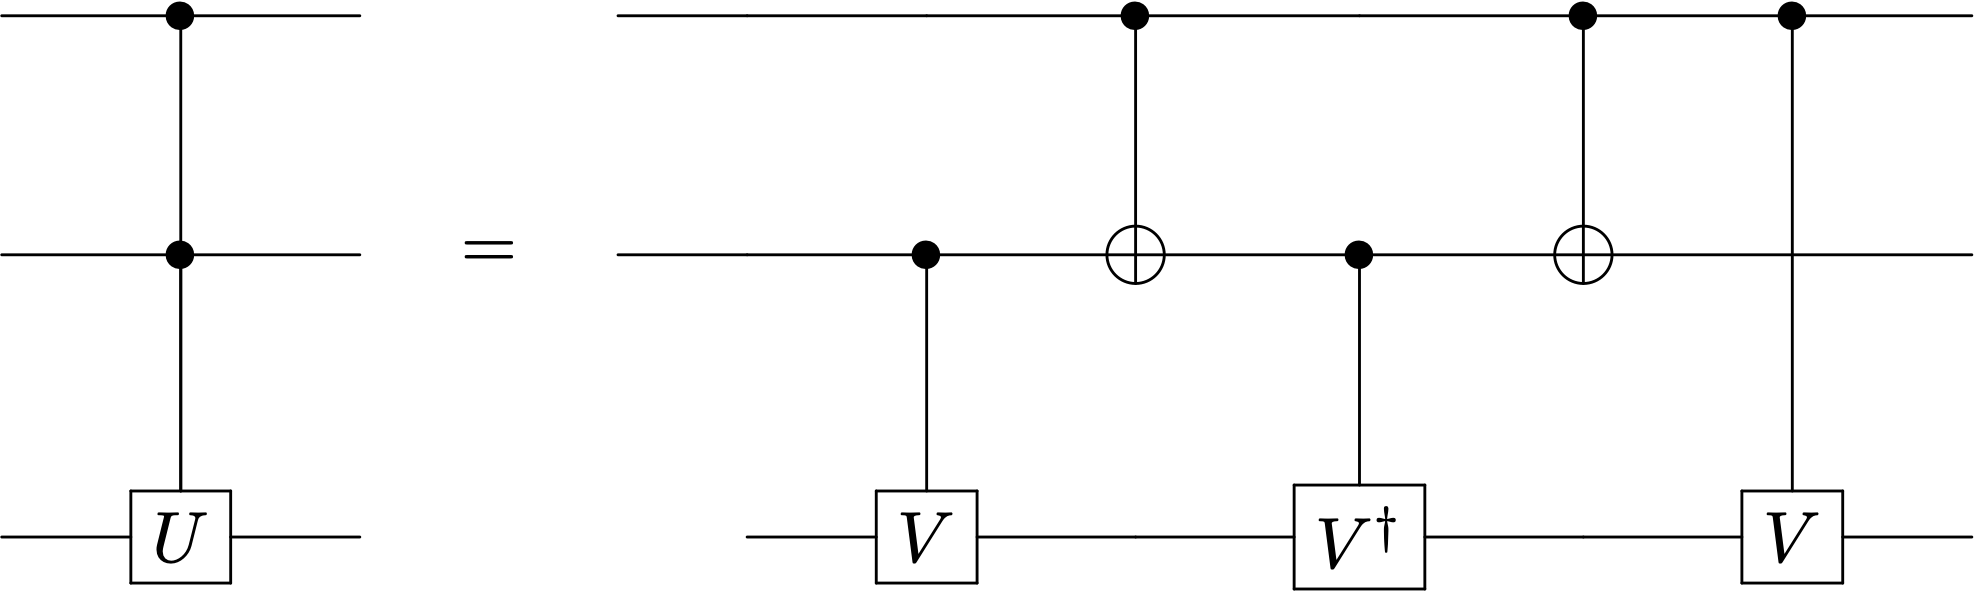
\includegraphics[width=0.60\linewidth]{Figuras/Fig_elementos_CCUdecomposition.png}
\caption{Desconposición de una puerta con dos controles}
\label{Fig_elementos_CCUdecomposition}
\end{figure}
Pista: puedes demostrarlo viendo que operaciones hacen ambos circuitos sobre el tercer qubit cuando por los dos
primeros entran los 4 estados posibles ($\ket{00}$, $\ket{10}$, $\ket{01}$ y $\ket{11}$)
}

\Ejercicio{
Competa los siguientes apartados:
\begin{itemize}
\item[1.] Programa y ejecuta un circuito de 16 cúbits que prepare el estado $\ket{00\ldots 0} \to \frac{1}{\sqrt{2}}\left(\ket{00\ldots 0} + \ket{11\ldots 1}\right) $
\item[2.] Modifica la posición de los controladores hasta reducir la profundidad a 5.
\end{itemize}
}

\Ejercicio{
\begin{itemize}
\item[a)]  Que es el quantum volume? Cuales son los procesadores con mayor Quantum Volume? Consulta las referencias:\\
\url{https://medium.com/qiskit/what-is-quantum-volume-anyway-a4dff801c36f}\\
\url{https://www.ibm.com/quantum/blog/quantum-volume-256}\\
\url{https://en.wikipedia.org/wiki/Quantum_volume}


\item[b)] IBM ya ha abandonado esta medida de calidad y ahora usa EPLG y CLOPS, que son estas medidas? Escribe una tabla con los procesadores que tiene IBM online gratuitos y sus valores EPLG y CLOPS. Consulta las referencias:\\
\url{https://www.ibm.com/quantum/blog/quantum-metric-layer-fidelity}\\
\url{https://quantum.ibm.com/services/resources}


\end{itemize}






}

\Ejercicio{
Completa el código del notebook para implementar la función $f:\{0,1\}^4\to \{0,1\}^4$ dada su tabla de verdad.
Recuerda que en qiskit el bit menos significativo es el de arriba.
}

\Ejercicio{
Escribe una función $f:S^n\to S$  que  produzca aleatoriamente $f(x) = \pm 1$ de forma \textit{equilibrada} (es decir, tantos $f(x)= +1$ como $f(x)= -1$).  Puedes ver la solución en la sección 4.4 de algoritmo de \href{https://learn.qiskit.org/course/ch-algorithms/deutsch-jozsa-algorithm}{Deutsch-Jozsa del notebook de Qiskit}.
}

\Ejercicio{
Completa el código del notebook que genera el circuito asociado a la función binaria lineal $f(x;a)$.
}

\Ejercicio{
Sea sobre el conjunto de valores $x\in \{0,1,2,3\}$ la función $f(x) = x^2$. Halla la tabla de verdad
en binario y construye el oráculo que implementa esta función.
}

\Ejercicio{
Oráculos constantes sólo hay dos, $f(x)=0~$ ó $~f(x) = 1$ para todo $x$. Oráculos equilibrados hay muchos. Construye un oráculo constante y uno
equilibrado. Construye el circuito de Deutsch-Josza y ponlo a prueba con estos dos oráculos. Para ello, sigue el tutorial del
\href{https://learn.qiskit.org/course/ch-algorithms/deutsch-jozsa-algorithm}{Notebook de Qiskit (https://learn.qiskit.org/course/ch-algorithms/deutsch-jozsa-algorithm)} .
}

\Ejercicio{
Completa el código del algoritmo de Simon en el notebook 08-Busqueda\_Oracula
}

\Ejercicio{
Utiliza la Ec. (\ref{ec_QFT_suma_nula}) para demostrar que, invirtiendo los signos de las fases obtenemos la QFT inversa. Es decir, demuestra que, si
\begin{equation}
U^{-1}_{QFT}\ket{x}  =  \frac{1}{\sqrt{N}}\sum_{y} e^{-2\pi i  xy /N} \ket{y}
\end{equation}
se sigue que
\begin{equation}
U_{QFT}^{-1}(U_{QFT} \ket{x}) ) \ket{x}
\end{equation}
Esto confirma que es un operador unitario $U_{QFT}^{-1} = U_{QFT}^\dagger$.
}

\Ejercicio{
Comprueba la veracidad de la ecuación (\ref{ec_Shor_suma_igual_1}) para el caso $a=7$ y $N=15$.
}

\end{document}